%%
%% This is file `sigconf.tex',
%% generated with the docstrip utility.
%%
%% The original source files were:
%%
%% samples.dtx  (with options: `all,proceedings,sigconf')
%%
%% IMPORTANT NOTICE:
%%
%% For the copyright see the source file.
%%
%% Any modified versions of this file must be renamed
%% with new filenames distinct from sigconf.tex.
%%
%% For distribution of the original source see the terms
%% for copying and modification in the file samples.dtx.
%%
%% This generated file may be distributed as long as the
%% original source files, as listed above, are part of the
%% same distribution. (The sources need not necessarily be
%% in the same archive or directory.)
%%
%%
%% Commands for TeXCount
%TC:macro \cite [option:text,text]
%TC:macro \citep [option:text,text]
%TC:macro \citet [option:text,text]
%TC:envir table 0 1
%TC:envir table* 0 1
%TC:envir tabular [ignore] word
%TC:envir displaymath 0 word
%TC:envir math 0 word
%TC:envir comment 0 0
%%
%% The first command in your LaTeX source must be the \documentclass
%% command.
%%
%% For submission and review of your manuscript please change the
%% command to \documentclass[manuscript, screen, review]{acmart}.
%%
%% When submitting camera ready or to TAPS, please change the command
%% to \documentclass[sigconf]{acmart} or whichever template is required
%% for your publication.
%%
%%
\documentclass[sigconf]{acmart}
%%
%% \BibTeX command to typeset BibTeX logo in the docs
\AtBeginDocument{%
  \providecommand\BibTeX{{%
    Bib\TeX}}}

%% Rights management information.  This information is sent to you
%% when you complete the rights form.  These commands have SAMPLE
%% values in them; it is your responsibility as an author to replace
%% the commands and values with those provided to you when you
%% complete the rights form.
\setcopyright{acmlicensed}
\copyrightyear{2018}
\acmYear{2018}
\acmDOI{XXXXXXX.XXXXXXX}
%% These commands are for a PROCEEDINGS abstract or paper.
\acmConference[Conference acronym 'XX]{Make sure to enter the correct
  conference title from your rights confirmation email}{June 03--05,
  2018}{Woodstock, NY}
%%
%%  Uncomment \acmBooktitle if the title of the proceedings is different
%%  from ``Proceedings of ...''!
%%
%%\acmBooktitle{Woodstock '18: ACM Symposium on Neural Gaze Detection,
%%  June 03--05, 2018, Woodstock, NY}
\acmISBN{978-1-4503-XXXX-X/2018/06}











% add usepackage by yma391
\usepackage[table]{xcolor}
\definecolor{lowerSimilarityBg}{RGB}{255,243,224}  % lower N--D similarity
\definecolor{higherSimilarityBg}{RGB}{227,242,253} % higher N--D similarity
\usepackage{siunitx}

\usepackage{enumitem}
% Query Schema
\usepackage{booktabs}
% \usepackage{amssymb}
\usepackage{graphicx}






%%
%% Submission ID.
%% Use this when submitting an article to a sponsored event. You'll
%% receive a unique submission ID from the organizers
%% of the event, and this ID should be used as the parameter to this command.
%%\acmSubmissionID{123-A56-BU3}

%%
%% For managing citations, it is recommended to use bibliography
%% files in BibTeX format.
%%
%% You can then either use BibTeX with the ACM-Reference-Format style,
%% or BibLaTeX with the acmnumeric or acmauthoryear sytles, that include
%% support for advanced citation of software artefact from the
%% biblatex-software package, also separately available on CTAN.
%%
%% Look at the sample-*-biblatex.tex files for templates showcasing
%% the biblatex styles.
%%
%%
%% The majority of ACM publications use numbered citations and
%% references.  The command \citestyle{authoryear} switches to the
%% "author year" style.
%%
%% If you are preparing content for an event
%% sponsored by ACM SIGGRAPH, you must use the "author year" style of
%% citations and references.
%% Uncommenting
%% the next command will enable that style.
%%\citestyle{acmauthoryear}


%%
%% end of the preamble, start of the body of the document source.
\begin{document}

%%
%% The "title" command has an optional parameter,
%% allowing the author to define a "short title" to be used in page headers.
\title{Normalization as a Safer Default for Property Graphs:
Evidence from TPC-H on Neo4j}
%%
%% The "author" command and its associated commands are used to define
%% the authors and their affiliations.
%% Of note is the shared affiliation of the first two authors, and the
%% "authornote" and "authornotemark" commands
%% used to denote shared contribution to the research.

%%
%% By default, the full list of authors will be used in the page
%% headers. Often, this list is too long, and will overlap
%% other information printed in the page headers. This command allows
%% the author to define a more concise list
%% of authors' names for this purpose.
\renewcommand{\shortauthors}{Trovato et al.}

%%
%% The abstract is a short summary of the work to be presented in the
%% article.
\begin{abstract}
  A clear and well-documented \LaTeX\ document is presented as an
  article formatted for publication by ACM in a conference proceedings
  or journal publication. Based on the ``acmart'' document class, this
  article presents and explains many of the common variations, as well
  as many of the formatting elements an author may use in the
  preparation of the documentation of their work.
\end{abstract}

%%
%% The code below is generated by the tool at http://dl.acm.org/ccs.cfm.
%% Please copy and paste the code instead of the example below.
%%
\begin{CCSXML}
<ccs2012>
 <concept>
  <concept_id>00000000.0000000.0000000</concept_id>
  <concept_desc>Do Not Use This Code, Generate the Correct Terms for Your Paper</concept_desc>
  <concept_significance>500</concept_significance>
 </concept>
 <concept>
  <concept_id>00000000.00000000.00000000</concept_id>
  <concept_desc>Do Not Use This Code, Generate the Correct Terms for Your Paper</concept_desc>
  <concept_significance>300</concept_significance>
 </concept>
 <concept>
  <concept_id>00000000.00000000.00000000</concept_id>
  <concept_desc>Do Not Use This Code, Generate the Correct Terms for Your Paper</concept_desc>
  <concept_significance>100</concept_significance>
 </concept>
 <concept>
  <concept_id>00000000.00000000.00000000</concept_id>
  <concept_desc>Do Not Use This Code, Generate the Correct Terms for Your Paper</concept_desc>
  <concept_significance>100</concept_significance>
 </concept>
</ccs2012>
\end{CCSXML}

\ccsdesc[500]{Do Not Use This Code~Generate the Correct Terms for Your Paper}
\ccsdesc[300]{Do Not Use This Code~Generate the Correct Terms for Your Paper}
\ccsdesc{Do Not Use This Code~Generate the Correct Terms for Your Paper}
\ccsdesc[100]{Do Not Use This Code~Generate the Correct Terms for Your Paper}

%%
%% Keywords. The author(s) should pick words that accurately describe
%% the work being presented. Separate the keywords with commas.
\keywords{Do, Not, Use, This, Code, Put, the, Correct, Terms, for,
  Your, Paper}


\received{20 February 2007}
\received[revised]{12 March 2009}
\received[accepted]{5 June 2009}

%%
%% This command processes the author and affiliation and title
%% information and builds the first part of the formatted document.
\maketitle

\begin{comment}
OLD VERSION
\paragraph{Update cost evaluation.}
We study whether normalization improves graph updates by avoiding attribute
replication induced by functional dependencies. In the normalized schema, each
attribute value is stored only once per key. By contrast, folding $X\rightarrow Y$
copies the attributes of $Y$ except its key into each referencing $X$, so every copy
must be updated. We consider eight TPC-H foreign key edges: $L\rightarrow PS$
($e_1$), $L\rightarrow O$ ($e_2$), $PS\rightarrow P$ ($e_3$),
$PS\rightarrow S$ ($e_4$), $O\rightarrow C$ ($e_5$), $C\rightarrow N$
($e_6$), $S\rightarrow N$ ($e_7$), and $N\rightarrow R$ ($e_8$). Their
subsets define $2^8=256$ schema variants. For each variant, selected relationships are folded, while the others are inherited by the resulting nodes. If a relation involved in a fold is still referenced by another relationship, its original node is retained. This ensures that the resulting schema is independent of fold order. We apply the same updates to the normalized
and folded schemas to isolate the effect of data duplication on update cost from
differences in the number of references to each key.
The normalized baseline and each folded variant use identical update cases and
corresponding key indexes. Only the terminal relation of each fold path is
updated, with all folded copies modified together. For update case $i$, $U_{D,i}$
and $U_{N,i}$ denote the update times in the folded and normalized schemas.
We report the minimum, median, and maximum of $U_D$ and compute
$\Delta_U=\operatorname{median}_i(U_{D,i}-U_{N,i})$. A positive
$\Delta_U$ indicates an advantage for normalization. We evaluate all variants
but report one representative for each distinct combination of a terminal relation
and the folds that cause its redundancy. All differences are computed as the folded schema minus the normalized schema. $\Delta_V$, $\Delta_E$, and $\Delta_P$ denote changes in the numbers of graph nodes, graph edges, and property cells, respectively. We also measure the one-time normalization cost of
rebuilding participating nodes, relationships, and indexes from folded data.

\end{comment}


\section{Experiments Evaluation} \label{sec:experiments}

Our evaluation asks three questions. First, how much does normalization reduce
update latency by eliminating replicated attributes (RQ1)? Second, how much query
time can de-normalization save, and is this saving commensurate with the cost
of constructing the corresponding de-normalized schema (RQ2)? Third, how does
normalization affect embedding similarity for records with the same or
different FD determinant values (RQ3)?

\subsection{Experimental Setup}

\paragraph{System and protocol.}
We run all experiments on a MacBook Pro running macOS~26.6, equipped with an
Apple M5 processor with 10 CPU cores and 16~GB of memory. We use
Neo4j~2026.06.0 on OpenJDK~21 and the Neo4j Python driver~6.2.0.
All comparisons use identical inputs and settings, and client-side wall-clock
time is reported separately from schema-transformation costs.

\paragraph{Schemas and datasets.}
\begin{table}[htbp]
\vspace{-10pt}
\centering
\setlength{\abovecaptionskip}{1pt}
\caption{Datasets used in the experiments.}
\label{tab:dataset_characteristics}
\resizebox{\columnwidth}{!}{%
\begin{tabular}{lrrrrrrrl}
\toprule
Dataset & $|V|$ & $|E|$ & $|P|$ & $|\mathcal{L}_V|$ & $|\mathcal{L}_E|$ & $|\mathcal{K}_V|$ & $|\mathcal{K}_E|$ & Type \\
\midrule
TPC-H & 866,602 & 1,527,169 & 11,666,267 & 8 & 8 & 61 & 0 & Synthetic \\
Offshore & 2,016,523 & 3,339,267 & 23,851,301 & 5 & 14 & 23 & 5 & Real-world \\
\bottomrule
\end{tabular}%
}
\vspace{-4pt}
\end{table}

Table~\ref{tab:dataset_characteristics} summarises the two evaluation datasets.
TPC-H is used for the update and query experiments, and Offshore for the
embedding experiments.
Here, $|V|$, $|E|$, and $|P|$ count nodes, relationships, and property values;
$|\mathcal{L}_V|$, $|\mathcal{L}_E|$, $|\mathcal{K}_V|$, and
$|\mathcal{K}_E|$ count node labels, relationship types, node property keys,
and relationship property keys.
In both graphs, records are nodes and fields are properties. TPC-H maps its
eight relations to \textsf{LINEITEM} ($L$), \textsf{PARTSUPP} ($PS$),
\textsf{PART} ($P$), \textsf{ORDERS} ($O$), \textsf{CUSTOMER} ($C$),
\textsf{SUPPLIER} ($S$), \textsf{NATION} ($N$), and \textsf{REGION} ($R$),
with foreign keys represented as directed relationships and Node Key
constraints enforcing primary keys. Offshore uses \textsf{ADDRESS} ($A$),
\textsf{ENTITY} ($E$), \textsf{INTERMEDIARY} ($I$), \textsf{OFFICER} ($OF$),
and \textsf{OTHER} ($OT$).


\subsection{Update Cost Evaluation}
We evaluate whether normalization reduces update cost by avoiding attribute
replication. For a foreign key edge $X\rightarrow Y$, de-normalization copies
the non-key attributes of $Y$ to every referencing $X$ node; updating $Y$
therefore requires all copies to be modified. We consider eight TPC-H edges:
$L\rightarrow PS$ ($e_1$), $L\rightarrow O$ ($e_2$),
$PS\rightarrow P$ ($e_3$), $PS\rightarrow S$ ($e_4$),
$O\rightarrow C$ ($e_5$), $C\rightarrow N$ ($e_6$),
$S\rightarrow N$ ($e_7$), and $N\rightarrow R$ ($e_8$).
Their subsets produce $2^8=256$ schema variants. Selected relationships are
de-normalized, while the remaining relationships are retained. A referenced
relation also remains as a node when required by another relationship, making
schema construction independent of processing order.

The normalized baseline and every de-normalized variant use identical update
cases and key indexes. Each case updates the terminal relation of a
de-normalization path and all copies derived from it. For case $i$, let
$U_{D,i}$ and $U_{N,i}$ denote the update times in the de-normalized and
normalized schemas. We report the minimum, median, and maximum of $U_D$, the
median of $U_N$, and the median paired difference
$\Delta_U=\operatorname{median}_i(U_{D,i}-U_{N,i})$. Because each matched case
is differenced before aggregation, $\Delta_U$ need not equal
$U_D^{\mathrm{med}}-U_N^{\mathrm{med}}$. A positive $\Delta_U$ favours
normalization. We report one representative for each distinct combination of
terminal relation and redundancy-inducing relationships. Finally,
$\Delta_V$, $\Delta_E$, and $\Delta_P$ measure changes in node, edge, and
property-cell counts, respectively, while normalization time captures the cost
of rebuilding the affected nodes, relationships, and indexes.




\begin{table}[htbp]
\centering
\caption{Update and normalization results for de-normalization strategies at SF = 0.1}
\label{tab:denorm_update_results}
\setlength{\tabcolsep}{2pt}
\resizebox{\columnwidth}{!}{
\begin{tabular}{ll
S[table-format=4.1,round-mode=places,round-precision=1]
S[table-format=4.1,round-mode=places,round-precision=1]
S[table-format=4.1,round-mode=places,round-precision=1]
S[table-format=3.1,round-mode=places,round-precision=1]
S[table-format=4.1,round-mode=places,round-precision=1]
S[table-format=2.1,round-mode=places,round-precision=1]
r r r}
\toprule
ID & Edge set &
\multicolumn{1}{c}{$U_D^{\min}$} &
\multicolumn{1}{c}{$U_D^{\mathrm{med}}$} &
\multicolumn{1}{c}{$U_D^{\max}$} &
$U_N^{\mathrm{med}}$ & $\Delta_U$ & \multicolumn{1}{c}{$B_N$} &
$\Delta_V$ & $\Delta_E$ & $\Delta_P$ \\
\midrule

\rowcolor{lightblue}
\multicolumn{11}{l}{\textit{Update target: PARTSUPP (PS)}} \\


$\mathrm{PS}_1$ & $\{e_1\}$
& 4.978 & 6.498 & 7.064 & 5.003 & +1.418 & 33.414046
& -80.0K & +440.6K & +1.40M \\

\midrule
\rowcolor{lightblue}
\multicolumn{11}{l}{\textit{Update target: ORDERS (O)}} \\


$\mathrm{O}_1$ & $\{e_2\}$
& 3.961 & 5.589 & 6.927 & 5.026 & +0.305 & 30.787963
& -150.0K & -150.0K & +3.45M \\

\midrule
\rowcolor{lightblue}
\multicolumn{11}{l}{\textit{Update target: PART (P)}} \\


$\mathrm{P}_1$ & $\{e_3\}$
& 5.011 & 5.980 & 6.045 & 5.449 & +0.235 & 9.075786
& -20.0K & -80.0K & +460.0K \\

$\mathrm{P}_2$ & $\{e_1,e_3\}$
& 5.126 & 7.982 & 8.859 & 5.449 & +2.084 & 31.669594
& -100.0K & -160.0K & +6.03M \\

\midrule
\rowcolor{lightblue}
\multicolumn{11}{l}{\textit{Update target: SUPPLIER (S)}} \\


$\mathrm{S}_1$ & $\{e_4\}$
& 4.001 & 6.994 & 8.050 & 5.949 & +1.080 & 7.311062
& -1.0K & -1.0K & +473.0K \\

$\mathrm{S}_2$ & $\{e_1,e_4\}$
& 6.855 & 9.284 & 10.982 & 5.949 & +3.739 & 30.214305
& -81.0K & +439.6K & +5.00M \\

\midrule
\rowcolor{lightblue}
\multicolumn{11}{l}{\textit{Update target: CUSTOMER (C)}} \\


$\mathrm{C}_1$ & $\{e_5\}$
& 4.994 & 7.147 & 8.226 & 5.405 & +1.943 & 7.747514
& -15.0K & -15.0K & +930.0K \\

$\mathrm{C}_2$ & $\{e_2,e_5\}$
& 5.858 & 8.864 & 11.035 & 5.405 & +3.132 & 30.312249
& -165.0K & -165.0K & +7.54M \\

\midrule
\rowcolor{lightblue}
\multicolumn{11}{l}{\textit{Update target: NATION (N)}} \\


$\mathrm{N}_1$ & $\{e_7\}$
& 4.585 & 5.962 & 8.091 & 5.991 & +0.106 & 0.809627
& 0 & 0 & +3.0K \\

$\mathrm{N}_2$ & $\{e_6\}$
& 7.070 & 11.015 & 13.586 & 5.991 & +5.095 & 2.760496
& 0 & 0 & +45.0K \\

$\mathrm{N}_3$ & $\{e_6,e_7\}$
& 6.127 & 9.304 & 11.798 & 5.991 & +3.626 & 3.053744
& -25 & -25 & +47.9K \\

$\mathrm{N}_4$ & $\{e_4,e_7\}$
& 10.312 & 13.960 & 17.878 & 5.991 & +8.164 & 7.396816
& -1.0K & -1.0K & +713.0K \\

$\mathrm{N}_5$ & $\{e_4,e_6,e_7\}$
& 13.297 & 17.005 & 22.537 & 5.991 & +11.114 & 10.233038
& -1.0K & -1.0K & +757.9K \\

$\mathrm{N}_6$ & $\{e_5,e_6\}$
& 20.447 & 26.002 & 49.778 & 5.991 & +20.011 & 8.045862
& -15.0K & -15.0K & +1.38M \\

$\mathrm{N}_7$ & $\{e_5,e_6,e_7\}$
& 20.710 & 27.154 & 35.218 & 5.991 & +21.266 & 10.832242
& -15.0K & -15.0K & +1.38M \\

$\mathrm{N}_8$ & $\{e_4,e_5,e_6,e_7\}$
& 27.511 & 37.086 & 46.618 & 5.991 & +31.241 & 17.547923
& -16.0K & -16.0K & +2.09M \\

$\mathrm{N}_9$ & $\{e_1,e_4,e_7\}$
& 60.771 & 88.601 & 122.287 & 5.991 & +82.617 & 27.949892
& -81.0K & +439.6K & +6.80M \\

$\mathrm{N}_{10}$ & $\{e_2,e_5,e_6\}$
& 74.062 & 97.953 & 110.305 & 5.991 & +92.466 & 28.865689
& -165.0K & -165.0K & +9.34M \\

$\mathrm{N}_{11}$ & $\{e_2,e_5,e_6,e_7\}$
& 74.352 & 98.743 & 114.504 & 5.991 & +92.829 & 33.406925
& -165.0K & -165.0K & +9.34M \\

$\mathrm{N}_{12}$ & $\{e_1,e_4,e_6,e_7\}$
& 62.896 & 92.685 & 132.842 & 5.991 & +87.101 & 33.969847
& -81.0K & +439.5K & +6.84M \\

$\mathrm{N}_{13}$ & $\{e_2,e_4,e_5,e_6,e_7\}$
& 80.880 & 108.799 & 123.035 & 5.991 & +102.788 & 35.612912
& -166.0K & -166.0K & +10.05M \\

$\mathrm{N}_{14}$ & $\{e_1,e_4,e_5,e_6,e_7\}$
& 73.890 & 112.681 & 148.331 & 5.991 & +107.214 & 37.938805
& -96.0K & +424.5K & +8.18M \\

$\mathrm{N}_{15}$ & $\{e_1,e_2,e_4,e_5,e_6,e_7\}$
& 182.081 & 242.725 & 648.917 & 5.991 & +237.067 & 56.319155
& -246.0K & +274.5K & +16.14M \\

\midrule
\rowcolor{lightblue}
\multicolumn{11}{l}{\textit{Update target: REGION (R)}} \\


$\mathrm{R}_1$ & $\{e_8\}$
& 4.016 & 5.588 & 7.010 & 5.972 & <0.1 & 0.388553
& -5 & -25 & +35 \\

$\mathrm{R}_2$ & $\{e_7,e_8\}$
& 5.449 & 9.142 & 12.046 & 5.972 & +3.142 & 0.974088
& -5 & -1.0K & +5.0K \\

$\mathrm{R}_3$ & $\{e_6,e_8\}$
& 10.929 & 12.977 & 15.875 & 5.972 & +7.099 & 1.665730
& -5 & -15.0K & +75.0K \\

$\mathrm{R}_4$ & $\{e_6,e_7,e_8\}$
& 11.034 & 13.450 & 30.860 & 5.972 & +7.913 & 2.383688
& -30 & -16.0K & +79.9K \\

$\mathrm{R}_5$ & $\{e_4,e_7,e_8\}$
& 37.697 & 41.849 & 59.384 & 5.972 & +35.861 & 8.594459
& -1.0K & -81.0K & +873.0K \\

$\mathrm{R}_6$ & $\{e_4,e_6,e_7,e_8\}$
& 42.789 & 50.413 & 105.095 & 5.972 & +44.650 & 10.802044
& -1.0K & -96.0K & +947.9K \\

$\mathrm{R}_7$ & $\{e_5,e_6,e_8\}$
& 76.404 & 93.532 & 129.638 & 5.972 & +88.177 & 9.933542
& -15.0K & -165.0K & +1.68M \\

$\mathrm{R}_8$ & $\{e_5,e_6,e_7,e_8\}$
& 75.168 & 89.640 & 127.438 & 5.972 & +84.015 & 10.418280
& -15.0K & -166.0K & +1.68M \\

$\mathrm{R}_9$ & $\{e_4,e_5,e_6,e_7,e_8\}$
& 108.573 & 135.399 & 198.270 & 5.972 & +129.687 & 19.132084
& -16.0K & -246.0K & +2.55M \\

$\mathrm{R}_{10}$ & $\{e_1,e_4,e_7,e_8\}$
& 338.044 & 405.243 & 622.647 & 5.972 & +400.049 & 38.041750
& -81.0K & -161.0K & +8.00M \\

$\mathrm{R}_{11}$ & $\{e_2,e_5,e_6,e_8\}$
& 344.405 & 468.253 & 618.003 & 5.972 & +462.297 & 39.453933
& -165.0K & -765.6K & +10.54M \\

$\mathrm{R}_{12}$ & $\{e_2,e_5,e_6,e_7,e_8\}$
& 353.687 & 443.244 & 590.725 & 5.972 & +437.271 & 40.950560
& -165.0K & -766.6K & +10.55M \\

$\mathrm{R}_{13}$ & $\{e_1,e_4,e_6,e_7,e_8\}$
& 317.009 & 400.160 & 548.114 & 5.972 & +394.163 & 39.849538
& -81.0K & -176.0K & +8.08M \\

$\mathrm{R}_{14}$ & $\{e_2,e_4,e_5,e_6,e_7,e_8\}$
& 401.710 & 500.963 & 687.057 & 5.972 & +494.988 & 42.839032
& -166.0K & -846.6K & +11.41M \\

$\mathrm{R}_{15}$ & $\{e_1,e_4,e_5,e_6,e_7,e_8\}$
& 412.792 & 513.665 & 725.645 & 5.972 & +508.184 & 44.646740
& -96.0K & -326.0K & +9.68M \\

$\mathrm{R}_{16}$ & $\{e_1,e_2,e_4,e_5,e_6,e_7,e_8\}$
& 799.664 & 995.374 & 2006.596 & 5.972 & +989.385 & 65.744367
& -246.0K & -926.6K & +18.54M \\

\bottomrule
\end{tabular}
}
\scriptsize
\textit{Note:} Update times and $\Delta_U$ are in ms; $B_N$ is the
one-time normalization cost in s. $\Delta_U$ is the median paired difference,
not the difference of medians. $\Delta_V$, $\Delta_E$, and $\Delta_P$ are
counts; $\mathrm{K}=10^3$ and $\mathrm{M}=10^6$.
\end{table}



At SF = 0.1, Table~\ref{tab:denorm_update_results} shows that normalized update
latency remains stable between 5.0 and 6.0~ms across the evaluated relations, while
denormalized update latency generally increases as attribute replication accumulates
along longer paths. All 39 reported cases have positive median paired
differences ($\Delta_U>0$), although $\Delta_U$ is only $0.01$~ms for
$e_8$ ($N\rightarrow R$). The largest benefit occurs for REGION
with $\{e_1,e_2,e_4,e_5,e_6,e_7,e_8\}$. This schema contains 18.54M additional property
cells, and its median update latency increases from 6.0 to 995.4~ms, resulting in
a 989.4~ms saving from normalization. As data replication increases, the time required
for normalization generally increases, from 0.4 to 65.7~s across the evaluated schemas.


\subsubsection{Case Study: Redundancy and Scale}
\paragraph{Effect of redundancy.}
We use NATION and REGION to examine how redundancy and data scale affect update
cost. They provide 15 and 16 representative denormalized schemas,
respectively; the other terminal relations have only one or two strategies.
The NATION strategies cover all choices along the paths
$L\rightarrow O\rightarrow C\rightarrow N$ and
$L\rightarrow PS\rightarrow S\rightarrow N$, and the REGION strategies extend
both paths with $N\rightarrow R$. At SF = 0.1, we compare the normalized schema
with every strategy using paired update group 8. We update
\texttt{n\_comment} for \texttt{n\_nationkey}=7 and \texttt{r\_comment} for
\texttt{r\_regionkey}=2; each latency is the median of ten repetitions.
Strategy IDs in both figures follow Table~\ref{tab:denorm_update_results}.

\begin{figure}[htbp]
    \centering
    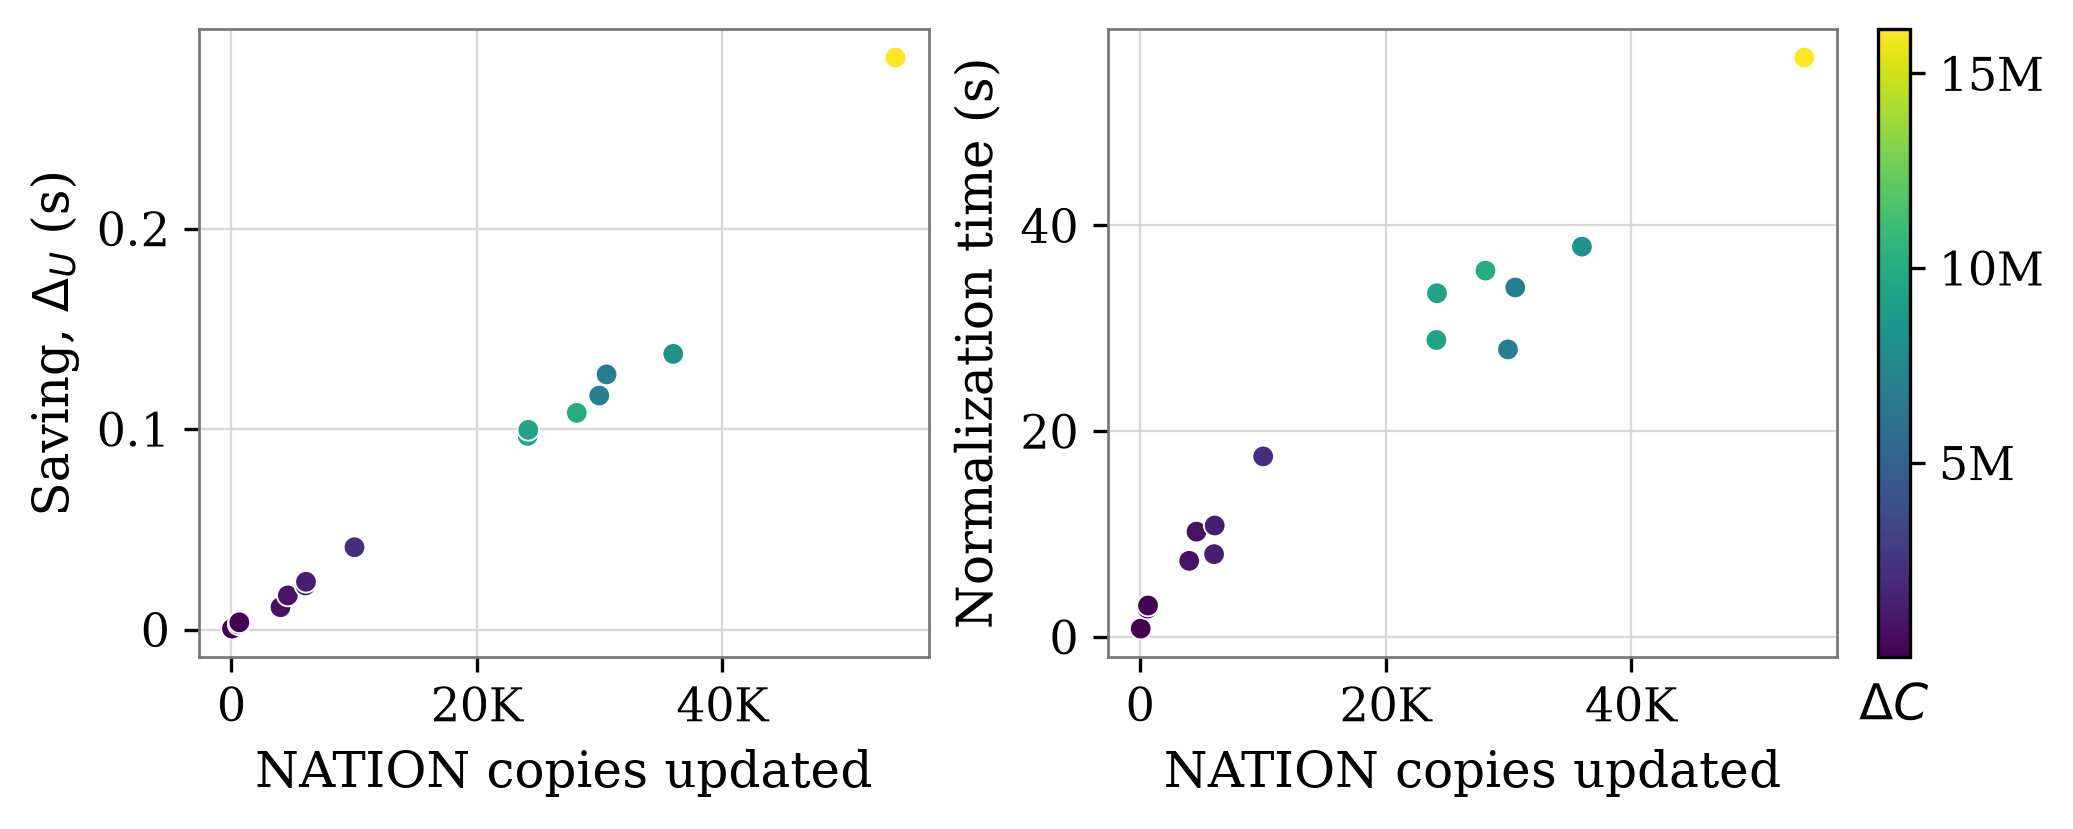
\includegraphics[width=0.47\textwidth]{figures/experiments/case_study_delta_vs_copies_nation.png}
    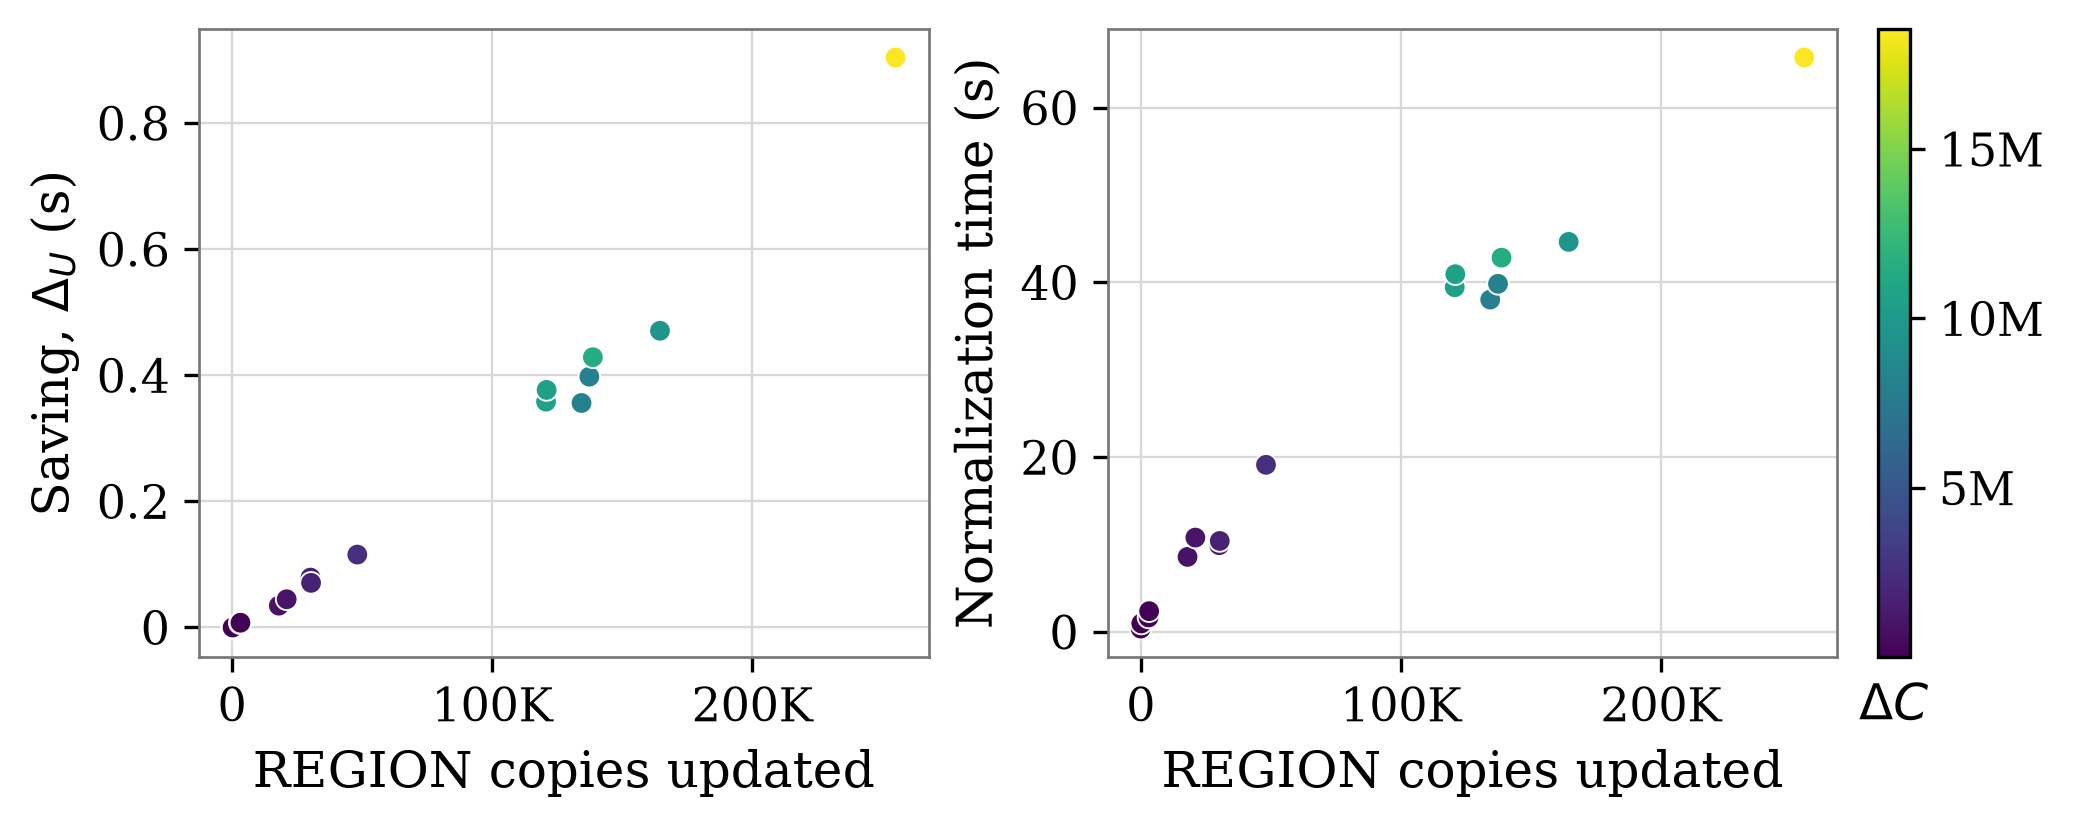
\includegraphics[width=0.47\textwidth]{figures/experiments/case_study_delta_vs_copies_region.png}
    \caption{NATION (upper pair) and REGION (lower pair) case studies at
    SF = 0.1, showing update-time saving (left), normalization cost
    (right), and additional property cells by colour.}
    \Description{NATION and REGION plots showing update-time saving and
    normalization cost by the number of copies updated; colour denotes
    additional property cells.}
    \label{fig:trade_off_schema}
\end{figure}



In Figure~\ref{fig:trade_off_schema}, the number of NATION copies ranges from
50 to 54.1K. Normalized latency is 5.5~ms, while denormalized latency ranges
from 6.0 to 290.9~ms, giving savings of 0.5 to 285.4~ms across all 15
strategies. For REGION, the number of copies ranges from 5 to 255.1K.
Normalized latency remains approximately 6~ms, while denormalized latency
ranges from 4~ms to 0.91~s. Strategies $\mathrm{R}_1$ and $\mathrm{R}_2$ have
differences of $-1.8$ and $-0.1$~ms; the remaining 14 strategies save 7.0 to
904.1~ms through normalization. At comparable copy counts of 137.4K and
138.7K, $\mathrm{R}_{13}$ and $\mathrm{R}_{14}$ contain 8.08M and 11.41M
additional cells and save 397.9 and 428.8~ms, respectively, showing that
$\Delta_P$ also affects update cost. The one-time normalization cost ranges
from 0.81 to 56.32~s for NATION and from 0.39 to 65.74~s for REGION.





\paragraph{Effect of scale.}
We compare the same 15 NATION and 16 REGION strategies at SF = 0.05, 0.1,
and 0.2, using all 50 paired update cases at each scale. Each case latency is
the median of ten repetitions. For each strategy, we report the median paired
normalization speedup $S_U=\operatorname{median}_i(U_{D,i}/U_{N,i})$ and the
one-time normalization cost. Each strategy uses the normalized baseline from
its own measurement run; values of $S_U>1$ favour normalization. The three SFs
span a fourfold increase in data scale, increasing replication along paths
through scale-dependent relations.

\begin{figure}[htbp]
    \centering
    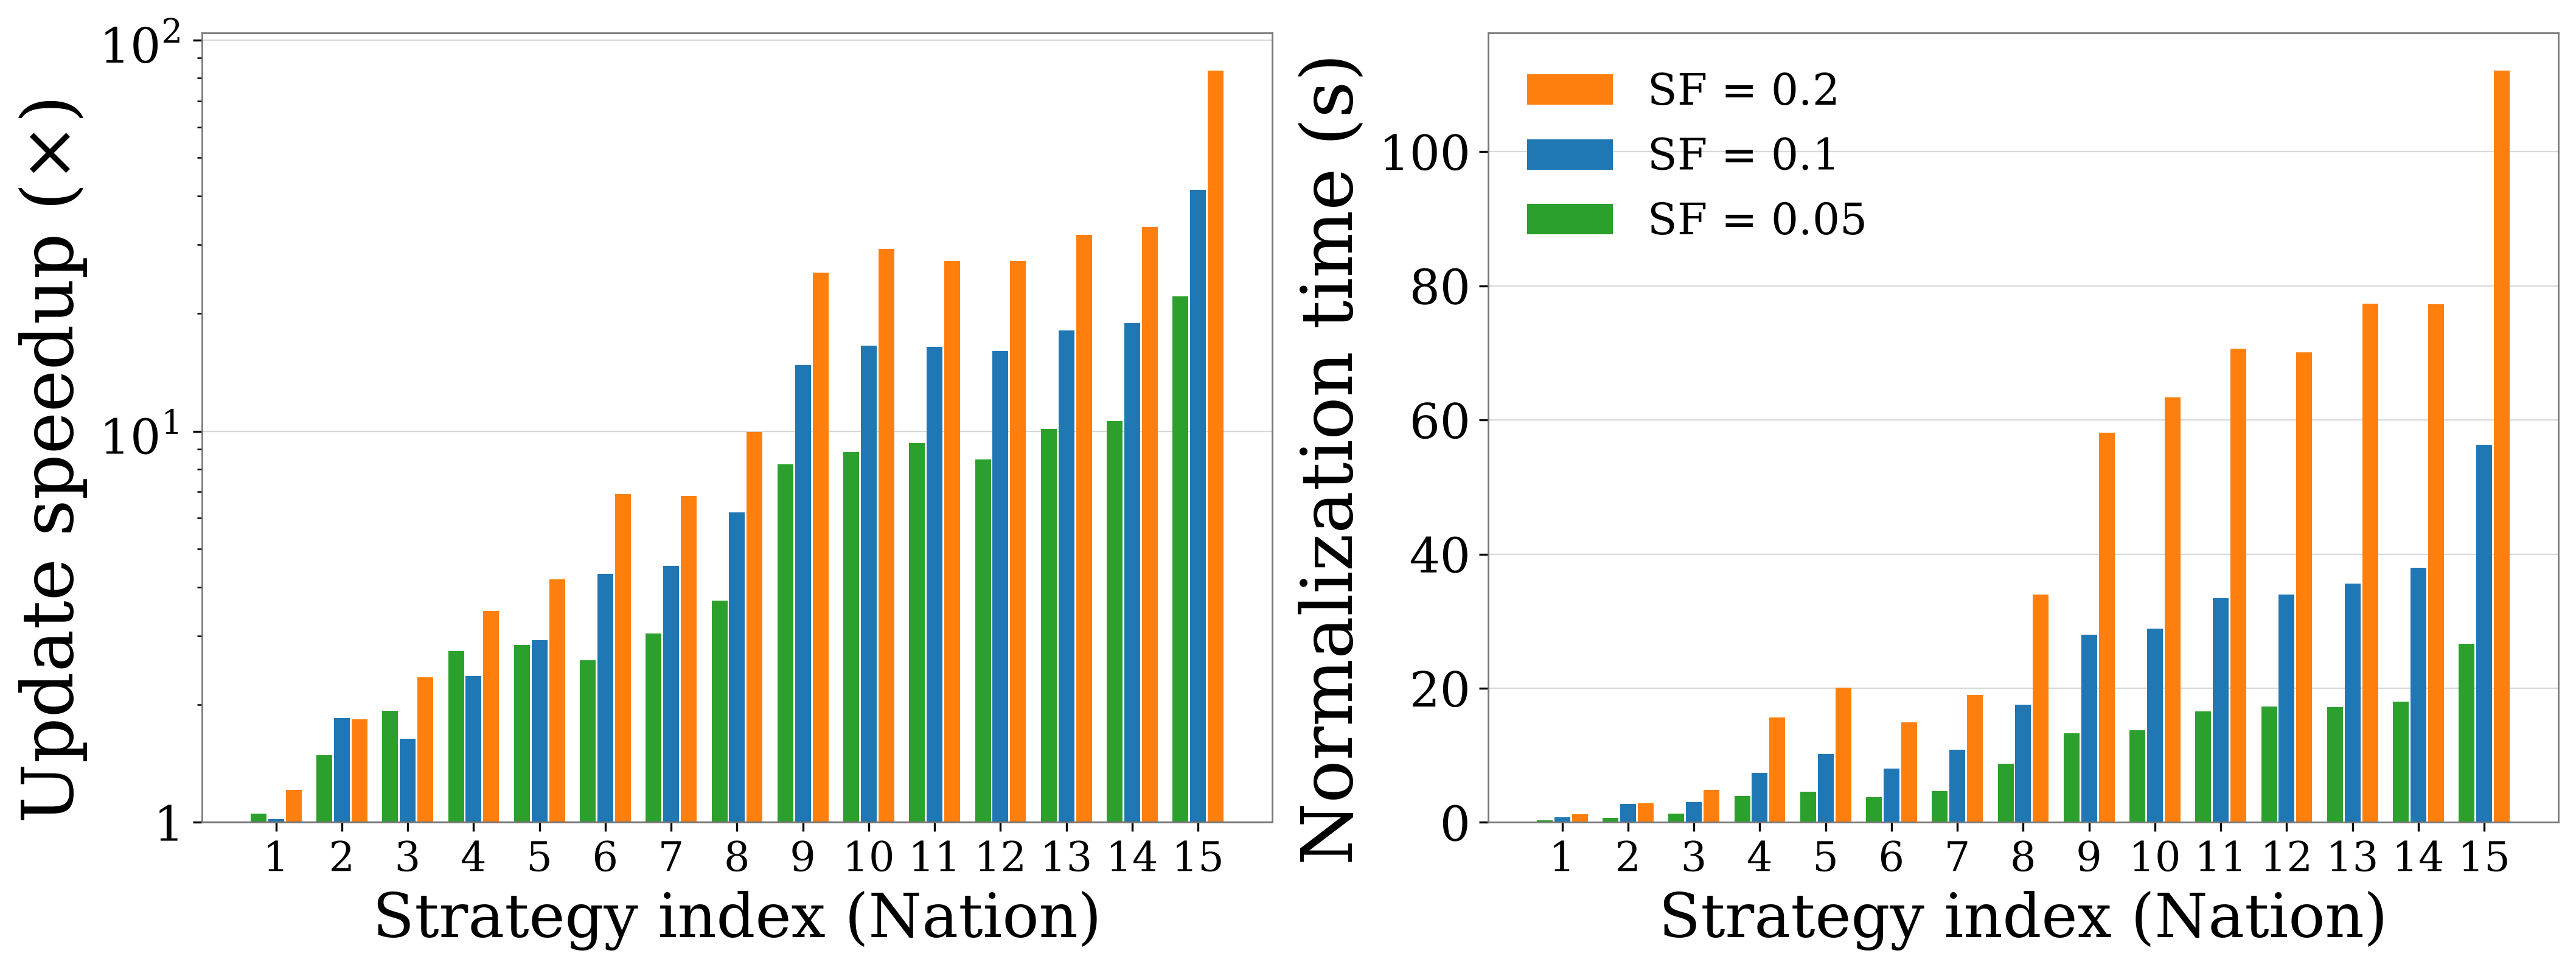
\includegraphics[width=\columnwidth]{figures/experiments/update_speedup_by_strategy_nation.png}
    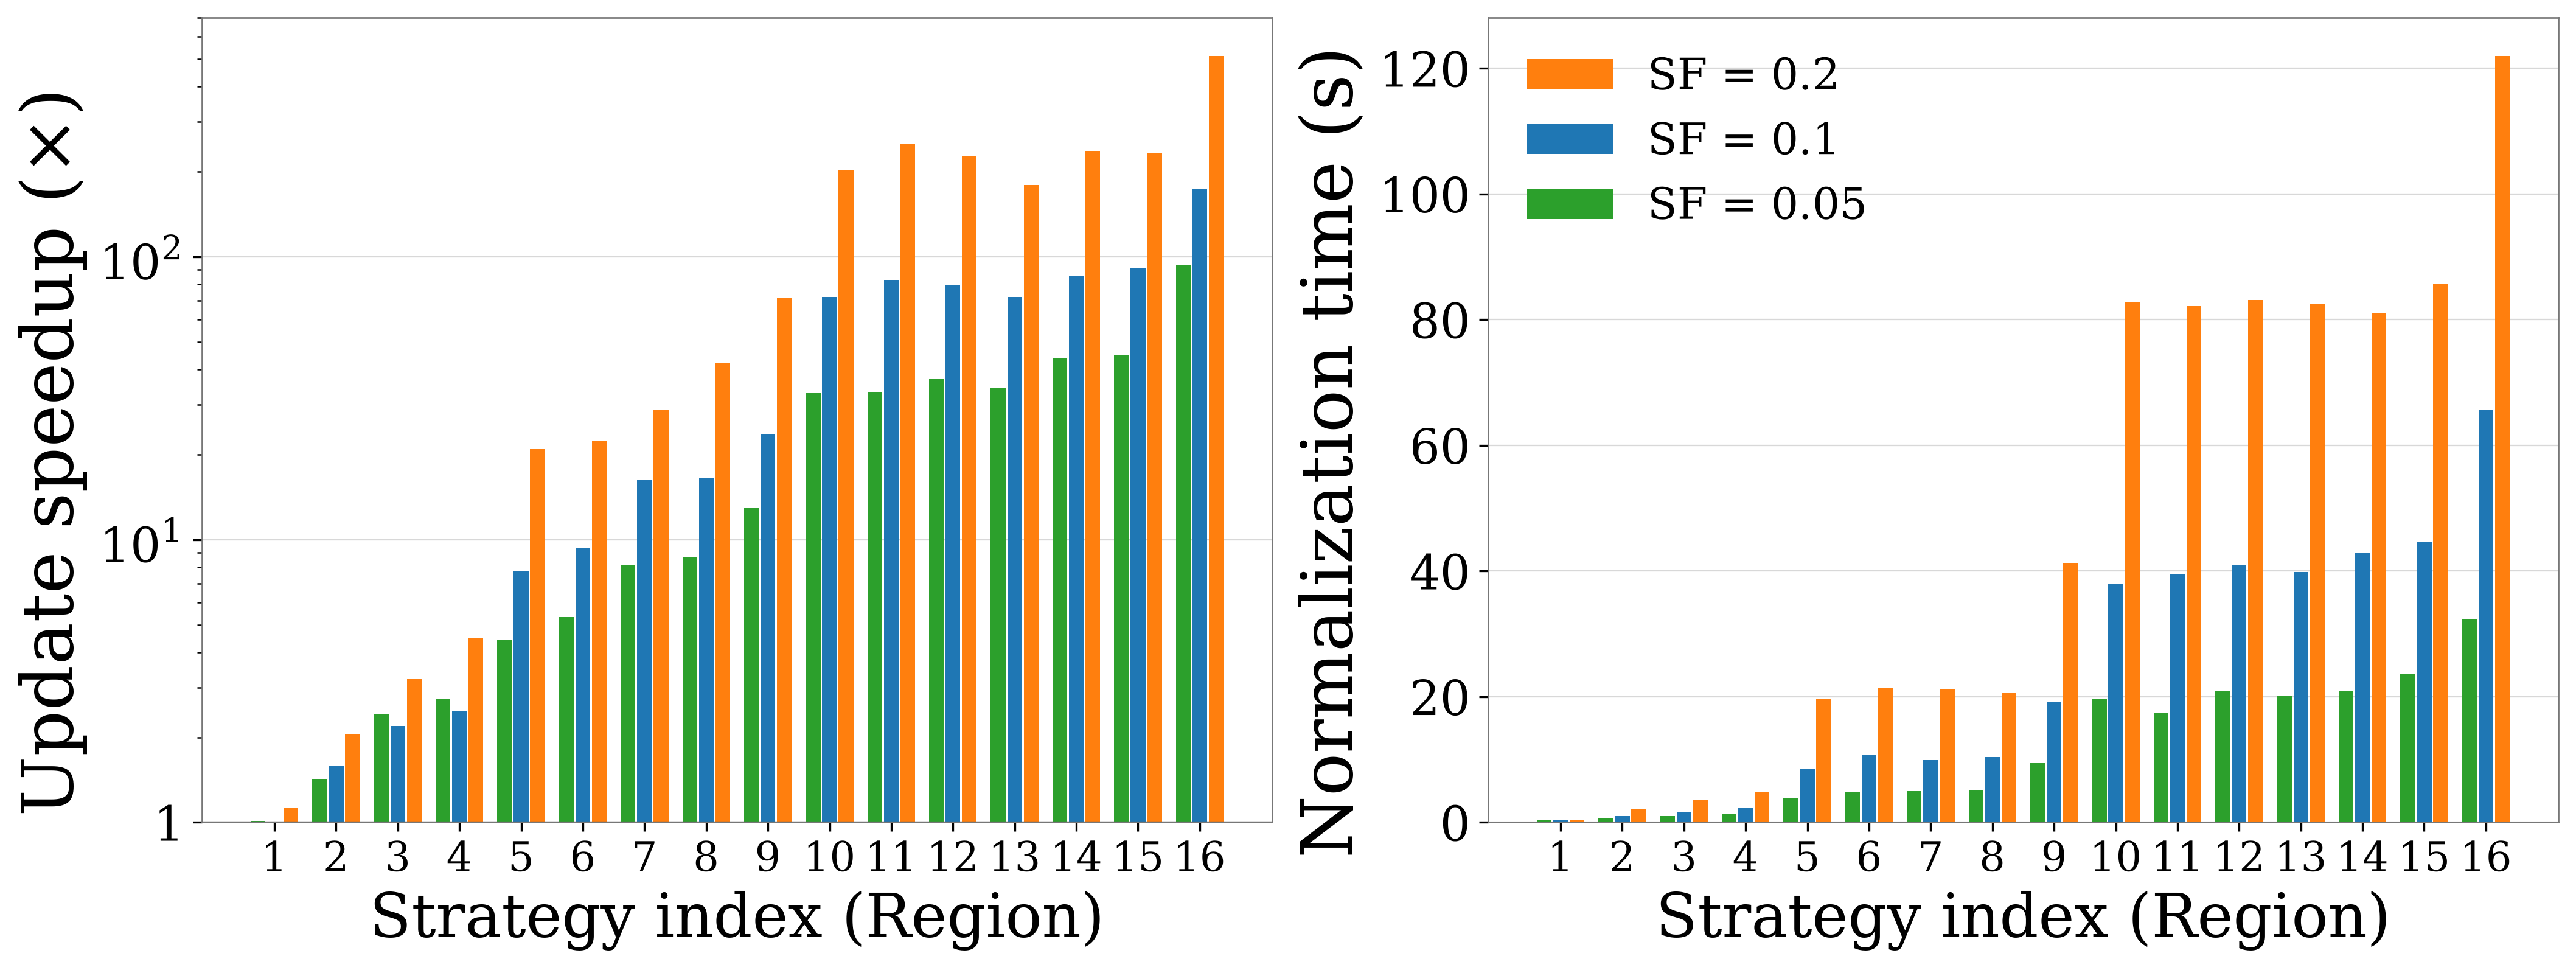
\includegraphics[width=\columnwidth]{figures/experiments/update_speedup_by_strategy_region.png}
    \caption{Effect of TPC-H scale factor on NATION (top) and REGION (bottom):
    median update speedup $S_U$ (left, log scale) and one-time normalization
    cost (right, linear scale).}
    \label{fig:sf_influence}
\end{figure}

Figure~\ref{fig:sf_influence} shows that increasing SF generally amplifies the
update benefit of normalization for strategies with substantial replication.
For NATION strategies $\mathrm{N}_9$--$\mathrm{N}_{15}$, median speedups span
$8.24$--$22.13\times$, $14.79$--$41.46\times$, and $25.42$--$83.58\times$
at SF = 0.05, 0.1, and 0.2, respectively. For REGION strategies
$\mathrm{R}_{10}$--$\mathrm{R}_{16}$, the corresponding ranges are
$32.99$--$93.84\times$, $72.07$--$173.64\times$, and
$179.81$--$512.94\times$. The trend is not monotonic for every strategy:
several strategies with little replication vary across SFs, and
$\mathrm{R}_1$ (NR) remains close to $1\times$.

For $\mathrm{R}_{16}$, increasing SF from 0.05 to 0.2 raises the additional
property-cell count from 9.26M to 37.04M and the median de-normalized update
latency from 515.1 to 2,242.5~ms. The corresponding normalized medians remain
between 4.2 and 6.0~ms across the three scales. The one-time normalization cost
for this strategy also grows, from 32.41~s at SF = 0.05 to 65.74~s at SF = 0.1
and 121.97~s at SF = 0.2. Greater scale therefore increases both the recurring
update benefit and the up-front normalization cost for this strategy.

\subsection{Limited Query Overhead of Normalization}

To assess the query-performance trade-off, we compare every de-normalization
strategy with the normalized schema at SF = 0.1. Strategies for the same query
use identical parameter sets and share one set of baseline measurements. Let
$T_D$ and $T_N$ denote the mean query times of the de-normalized and normalized
schemas, respectively. We define $\Delta_D=T_N-T_D>0$ when de-normalization is
faster and $\Delta_N=T_D-T_N>0$ when normalization is faster.
Each de-normalized run uses a server-side timeout set to twice the normalized
runtime for the same parameters. Timed-out runs are marked as \emph{capped},
with the timeout threshold used as a runtime lower bound.
After excluding strategies with capped runs,
Table~\ref{tab:query_advantage_comparison} shows the largest
exact gain for each applicable query in both directions. Let $B_D$ denote the
time in seconds required to construct the selected de-normalized schema. For
$\Delta_D>0$, we define
$\kappa=\lceil 1000B_D/\Delta_D\rceil$, the minimum number of
repeated query executions required to amortise construction.



\begin{table}[t]
\centering
\caption{Largest query-time gains at SF = 0.1: normalized baselines (left) and de-normalized strategies (right).}
\label{tab:query_advantage_comparison}
\begin{minipage}[t]{0.49\columnwidth}
\vspace{0pt}
\centering
\resizebox{\linewidth}{!}{%
\begin{tabular}{S[table-format=2.0] l
S[table-format=3.1,round-mode=places,round-precision=1]
S[table-format=3.1,round-mode=places,round-precision=1]
S[table-format=3.1,round-mode=places,round-precision=1]
S[table-format=2.1,round-mode=places,round-precision=1]}
\toprule
\multicolumn{1}{c}{Q} & Edge set &
\multicolumn{1}{c}{$T_D$} & \multicolumn{1}{c}{$T_N$} &
\multicolumn{1}{c}{$\Delta_N$} & \multicolumn{1}{c}{Build} \\
\midrule
5 & $\{e_2\}$ & 58.709 & 34.284 & 24.425 & 21.057 \\
7 & $\{e_7\}$ & 44.318 & 34.355 & 9.963 & 0.590 \\
8 & $\{e_2\}$ & 79.752 & 62.961 & 16.792 & 21.645 \\
9 & $\{e_7\}$ & 93.806 & 55.807 & 37.999 & 0.652 \\
10 & $\{e_6\}$ & 65.692 & 40.417 & 25.275 & 2.993 \\
11 & $\{e_4,e_7\}$ & 27.998 & 4.680 & 23.317 & 19.338 \\
12 & $\{e_2\}$ & 152.585 & 131.120 & 21.465 & 21.087 \\
13 & $\{e_5\}$ & 120.581 & 108.419 & 12.161 & 7.682 \\
16 & $\{e_3,e_4\}$ & 116.615 & 54.042 & 62.573 & 7.826 \\
18 & $\{e_2\}$ & 402.401 & 223.565 & 178.836 & 20.961 \\
20 & $\{e_1,e_3,e_4\}$ & 14.059 & 9.129 & 4.931 & 37.810 \\
22 & $\{e_5\}$ & 36.149 & 19.013 & 17.135 & 7.488 \\
\bottomrule
\end{tabular}%
}
\end{minipage}\hfill
\begin{minipage}[t]{0.49\columnwidth}
\vspace{0pt}
\centering
\resizebox{\linewidth}{!}{%
\begin{tabular}{S[table-format=2.0] l
S[table-format=3.1,round-mode=places,round-precision=1]
S[table-format=3.1,round-mode=places,round-precision=1]
S[table-format=3.1,round-mode=places,round-precision=1]
S[table-format=2.1,round-mode=places,round-precision=1]
S[table-format=4.0]}
\toprule
\multicolumn{1}{c}{Q} & Edge set &
\multicolumn{1}{c}{$T_D$} & \multicolumn{1}{c}{$T_N$} &
\multicolumn{1}{c}{$\Delta_D$} & \multicolumn{1}{c}{Build} &
\multicolumn{1}{c}{$\kappa$} \\
\midrule
2 & $\{e_4,e_7,e_8\}$ & 7.702 & 22.022 & 14.319 & 19.710 & 1377 \\
3 & $\{e_5\}$ & 48.179 & 75.784 & 27.604 & 8.239 & 299 \\
5 & $\{e_5\}$ & 32.159 & 34.284 & 2.126 & 7.990 & 3759 \\
7 & $\{e_2,e_5\}$ & 26.419 & 34.355 & 7.936 & 27.312 & 3442 \\
8 & $\{e_5\}$ & 46.563 & 62.961 & 16.397 & 7.114 & 434 \\
9 & $\{e_1,e_2\}$ & 44.589 & 55.807 & 11.218 & 27.493 & 2451 \\
20 & $\{e_3,e_4\}$ & 5.796 & 9.129 & 3.333 & 7.135 & 2141 \\
21 & $\{e_7\}$ & 42.249 & 52.071 & 9.822 & 0.610 & 63 \\
\bottomrule
\end{tabular}%
}
\vspace{2pt}

{\scriptsize\raggedright
\textit{Note:} Rows show maximum $\Delta_N=T_D-T_N$ (left) or
$\Delta_D=T_N-T_D$ (right). Times are in ms; Build is in s, and
$\kappa$ is the break-even query count.\par}
\end{minipage}
\end{table}



Among the 74 strategies, 44 favour normalization: 28 are exact cases across 12
queries, and 16 contain capped runs whose lower-bound means still exceed the
baseline. The left panel gives the largest
exact gain per query (4.9--178.8~ms; median 22.4~ms), led by Q18 with
$\{e_2\}$. The remaining 30 exact strategies favour de-normalization across
eight queries; the right panel gives the largest gain per query
(2.1--27.6~ms; median 10.5~ms), led by Q3 with $\{e_5\}$. The corresponding
schemas take 0.6--37.8~s and 0.6--27.5~s to build, respectively. Thus,
the eight de-normalization gains require 63--3,759 executions to amortise
construction (median 1,759), and five require more than 1,000. These optimistic
estimates exclude subsequent maintenance. Normalization can therefore provide
larger gains, whereas de-normalization yields only modest query-time
improvements with substantial amortisation requirements.



\subsection{Graph Embedding Evaluation}

We evaluate 12 FDs within individual Offshore node types: nine strict and three
approximate. For an FD $X\rightarrow Y$, the de-normalized graph retains $X$
and $Y$ on each source node, whereas normalization places them on a dimension
node shared by source nodes with the same $X$ value. Groups with missing or
conflicting values are excluded.

For each of ten seeds, we sample up to 1,000 pairs of source nodes that share
an $X$ value and an equal number that do not. We fix the sampled pairs, seeds,
feature construction procedure, and algorithm settings across representations.
Embeddings have 128 dimensions, and all relationships are projected as
undirected. Property Hash uses node properties only, Node2Vec uses graph
structure only, and FastRP, HashGNN, and GraphSAGE combine both. For each pair
set, Table~\ref{tab:offshore_embedding_determinant_comparison} reports the mean
of the median cosine similarities from the ten seeds. Higher similarity is
desirable for pairs with the same determinant value and lower similarity for
pairs with different determinant values.


\begin{table*}[t]
\centering
\caption{Cosine similarity for 12 Offshore functional dependency cases under
an undirected projection.}
\label{tab:offshore_embedding_determinant_comparison}
\newcommand{\highscore}[1]{%
    \multicolumn{1}{c}{\cellcolor{higherSimilarityBg}\bfseries #1}}
\newcommand{\lowscore}[1]{%
    \multicolumn{1}{c}{\cellcolor{lowerSimilarityBg}\bfseries #1}}
\newcommand{\fdattr}[1]{\mathit{#1}}
\resizebox{\textwidth}{!}{%
\begin{tabular}{@{}cll *{10}{S[table-format=1.3]}@{}}
\toprule
ID & Node type & FD
& \multicolumn{1}{c}{$\mathrm{PH}_{N}$}
& \multicolumn{1}{c}{$\mathrm{PH}_{D}$}
& \multicolumn{1}{c}{$\mathrm{FRP}_{N}$}
& \multicolumn{1}{c}{$\mathrm{FRP}_{D}$}
& \multicolumn{1}{c}{$\mathrm{N2V}_{N}$}
& \multicolumn{1}{c}{$\mathrm{N2V}_{D}$}
& \multicolumn{1}{c}{$\mathrm{HGN}_{N}$}
& \multicolumn{1}{c}{$\mathrm{HGN}_{D}$}
& \multicolumn{1}{c}{$\mathrm{GS}_{N}$}
& \multicolumn{1}{c}{$\mathrm{GS}_{D}$} \\
\midrule
\multicolumn{13}{@{}l}{\textbf{Pairs Sharing the Same Determinant Value}} \\
\midrule
1 & Address & $\fdattr{countries} \rightarrow \fdattr{country\_codes}$ & 0.478 & \highscore{0.559} & \highscore{0.723} & 0.294 & \highscore{0.998} & 0.511 & \highscore{0.639} & 0.593 & \highscore{0.975} & 0.959 \\
2 & Entity & $\fdattr{service\_provider} \rightarrow \{\fdattr{sourceID},\,\fdattr{valid\_until}\}$ & 0.204 & \highscore{0.419} & \highscore{0.488} & 0.388 & \highscore{0.553} & 0.551 & \highscore{0.558} & 0.552 & 0.975 & \highscore{0.990} \\
3 & Entity & $\fdattr{country\_codes} \rightarrow \fdattr{countries}$ & 0.684 & \highscore{0.734} & \highscore{0.729} & 0.612 & \highscore{0.706} & 0.595 & 0.688 & \highscore{0.689} & \highscore{0.997} & 0.995 \\
4 & Entity & $\fdattr{countries} \rightarrow \fdattr{country\_codes}$ & 0.685 & \highscore{0.731} & \highscore{0.728} & 0.612 & \highscore{0.704} & 0.597 & \highscore{0.704} & 0.660 & \highscore{0.996} & 0.994 \\
5 & Intermediary & $\fdattr{country\_codes} \rightarrow \fdattr{countries}$ & 0.503 & \highscore{0.562} & \highscore{0.541} & 0.273 & \highscore{0.998} & 0.641 & \highscore{0.628} & 0.550 & 0.946 & \highscore{0.974} \\
6 & Intermediary & $\fdattr{countries} \rightarrow \fdattr{country\_codes}$ & 0.503 & \highscore{0.557} & \highscore{0.545} & 0.275 & \highscore{0.998} & 0.670 & \highscore{0.622} & 0.561 & \highscore{0.977} & 0.954 \\
7 & Intermediary & $\fdattr{valid\_until} \rightarrow \fdattr{sourceID}$ & 0.034 & \highscore{0.754} & 0.426 & \highscore{0.432} & \highscore{0.997} & 0.733 & 0.588 & \highscore{0.650} & 0.988 & \highscore{0.988} \\
8 & Intermediary & $\fdattr{sourceID} \rightarrow \fdattr{valid\_until}$ & 0.153 & \highscore{0.748} & \highscore{0.441} & 0.432 & \highscore{0.997} & 0.698 & 0.577 & \highscore{0.632} & 0.982 & \highscore{0.990} \\
9 & Other & $\fdattr{jurisdiction} \rightarrow \fdattr{jurisdiction\_description}$ & 0.689 & \highscore{0.744} & \highscore{0.543} & 0.421 & \highscore{0.998} & 0.397 & \highscore{0.691} & 0.652 & \highscore{0.967} & 0.939 \\
10 & Other & $\fdattr{jurisdiction\_description} \rightarrow \fdattr{jurisdiction}$ & 0.689 & \highscore{0.728} & \highscore{0.530} & 0.405 & \highscore{0.998} & 0.397 & \highscore{0.668} & 0.655 & \highscore{0.966} & 0.937 \\
11 & Other & $\fdattr{country\_codes} \rightarrow \fdattr{countries}$ & 0.717 & \highscore{0.777} & \highscore{0.641} & 0.384 & 0.506 & \highscore{0.526} & \highscore{0.714} & 0.637 & \highscore{0.981} & 0.973 \\
12 & Other & $\fdattr{countries} \rightarrow \fdattr{country\_codes}$ & 0.716 & \highscore{0.780} & \highscore{0.631} & 0.373 & 0.509 & \highscore{0.523} & \highscore{0.711} & 0.641 & \highscore{0.987} & 0.975 \\
\midrule
\multicolumn{13}{@{}l}{\textbf{Pairs with Different Determinant Values}} \\
\midrule
1 & Address & $\fdattr{countries} \rightarrow \fdattr{country\_codes}$ & 0.232 & \lowscore{0.202} & 0.190 & \lowscore{0.131} & \lowscore{0.407} & 0.506 & 0.486 & \lowscore{0.485} & 0.701 & \lowscore{0.687} \\
2 & Entity & $\fdattr{service\_provider} \rightarrow \{\fdattr{sourceID},\,\fdattr{valid\_until}\}$ & \lowscore{0.058} & 0.122 & 0.127 & \lowscore{0.110} & 0.523 & \lowscore{0.522} & 0.485 & \lowscore{0.476} & 0.450 & \lowscore{0.447} \\
3 & Entity & $\fdattr{country\_codes} \rightarrow \fdattr{countries}$ & 0.211 & \lowscore{0.187} & 0.164 & \lowscore{0.147} & \lowscore{0.487} & 0.511 & 0.513 & \lowscore{0.505} & 0.774 & \lowscore{0.680} \\
4 & Entity & $\fdattr{countries} \rightarrow \fdattr{country\_codes}$ & 0.210 & \lowscore{0.196} & 0.166 & \lowscore{0.148} & \lowscore{0.488} & 0.513 & 0.533 & \lowscore{0.469} & 0.644 & \lowscore{0.644} \\
5 & Intermediary & $\fdattr{country\_codes} \rightarrow \fdattr{countries}$ & 0.371 & \lowscore{0.316} & 0.216 & \lowscore{0.148} & \lowscore{0.462} & 0.617 & 0.539 & \lowscore{0.480} & \lowscore{0.750} & 0.845 \\
6 & Intermediary & $\fdattr{countries} \rightarrow \fdattr{country\_codes}$ & 0.373 & \lowscore{0.317} & 0.217 & \lowscore{0.148} & \lowscore{0.475} & 0.653 & 0.531 & \lowscore{0.488} & 0.884 & \lowscore{0.804} \\
7 & Intermediary & $\fdattr{valid\_until} \rightarrow \fdattr{sourceID}$ & \lowscore{0.000} & 0.263 & \lowscore{0.110} & 0.138 & \lowscore{0.400} & 0.625 & 0.502 & \lowscore{0.502} & 0.925 & \lowscore{0.822} \\
8 & Intermediary & $\fdattr{sourceID} \rightarrow \fdattr{valid\_until}$ & \lowscore{0.000} & 0.275 & \lowscore{0.128} & 0.163 & \lowscore{0.388} & 0.569 & \lowscore{0.490} & 0.503 & 0.845 & \lowscore{0.805} \\
9 & Other & $\fdattr{jurisdiction} \rightarrow \fdattr{jurisdiction\_description}$ & 0.131 & \lowscore{0.094} & 0.067 & \lowscore{0.057} & 0.467 & \lowscore{0.442} & 0.481 & \lowscore{0.420} & 0.875 & \lowscore{0.676} \\
10 & Other & $\fdattr{jurisdiction\_description} \rightarrow \fdattr{jurisdiction}$ & \lowscore{0.129} & 0.160 & 0.106 & \lowscore{0.089} & 0.463 & \lowscore{0.443} & 0.465 & \lowscore{0.433} & 0.873 & \lowscore{0.844} \\
11 & Other & $\fdattr{country\_codes} \rightarrow \fdattr{countries}$ & 0.705 & \lowscore{0.527} & 0.413 & \lowscore{0.293} & \lowscore{0.481} & 0.502 & 0.591 & \lowscore{0.549} & 0.851 & \lowscore{0.615} \\
12 & Other & $\fdattr{countries} \rightarrow \fdattr{country\_codes}$ & 0.701 & \lowscore{0.510} & 0.405 & \lowscore{0.280} & \lowscore{0.482} & 0.507 & 0.593 & \lowscore{0.547} & 0.919 & \lowscore{0.619} \\
\bottomrule
\end{tabular}%
}
\vspace{1pt}
\begin{center}
    \scriptsize
    \textit{Note:} PH = Property Hash, FRP = FastRP, N2V = Node2Vec,
    HGN = HashGNN, GS = GraphSAGE; N/D = normalized/de-normalized.
    Values are means of the median similarities from 10 seeds (three decimals).
    Light blue (orange) highlights the higher (lower) similarity between
    N and D for same (different) determinant values, based on unrounded
    results. The two panels use the same IDs.
\end{center}
\end{table*}

\paragraph{Similarity scores.}
The reported similarity is higher for pairs with the same determinant value
than for pairs with different determinant values in 118 of the 120 combinations
of representation, method, and FD. The embeddings therefore retain the
determinant grouping in almost every case. Property Hash favours
de-normalization in all 12 comparisons for pairs with the same determinant
value because it cannot aggregate the features stored on dimension nodes after
normalization moves $X$ and $Y$ there. Among the four methods that use graph
structure, normalization increases similarity for pairs with the same
determinant value in 38 of 48 comparisons, but also increases it for pairs with
different determinant values in 35 of 48. We therefore compare the gap between
the two pair sets rather than either score alone.

\paragraph{Determinant separation.}
The similarity gap between pairs with the same and different determinant
values provides a more direct measure of determinant grouping. Across the four
methods that use graph structure, normalization increases the average gap from
0.172 to 0.269 and produces the larger gap in 32 of the 48 combinations of
method and FD. The effect holds for every FastRP and Node2Vec FD, but is less
consistent for HashGNN and GraphSAGE.

\begin{figure}[htbp]
    \centering
    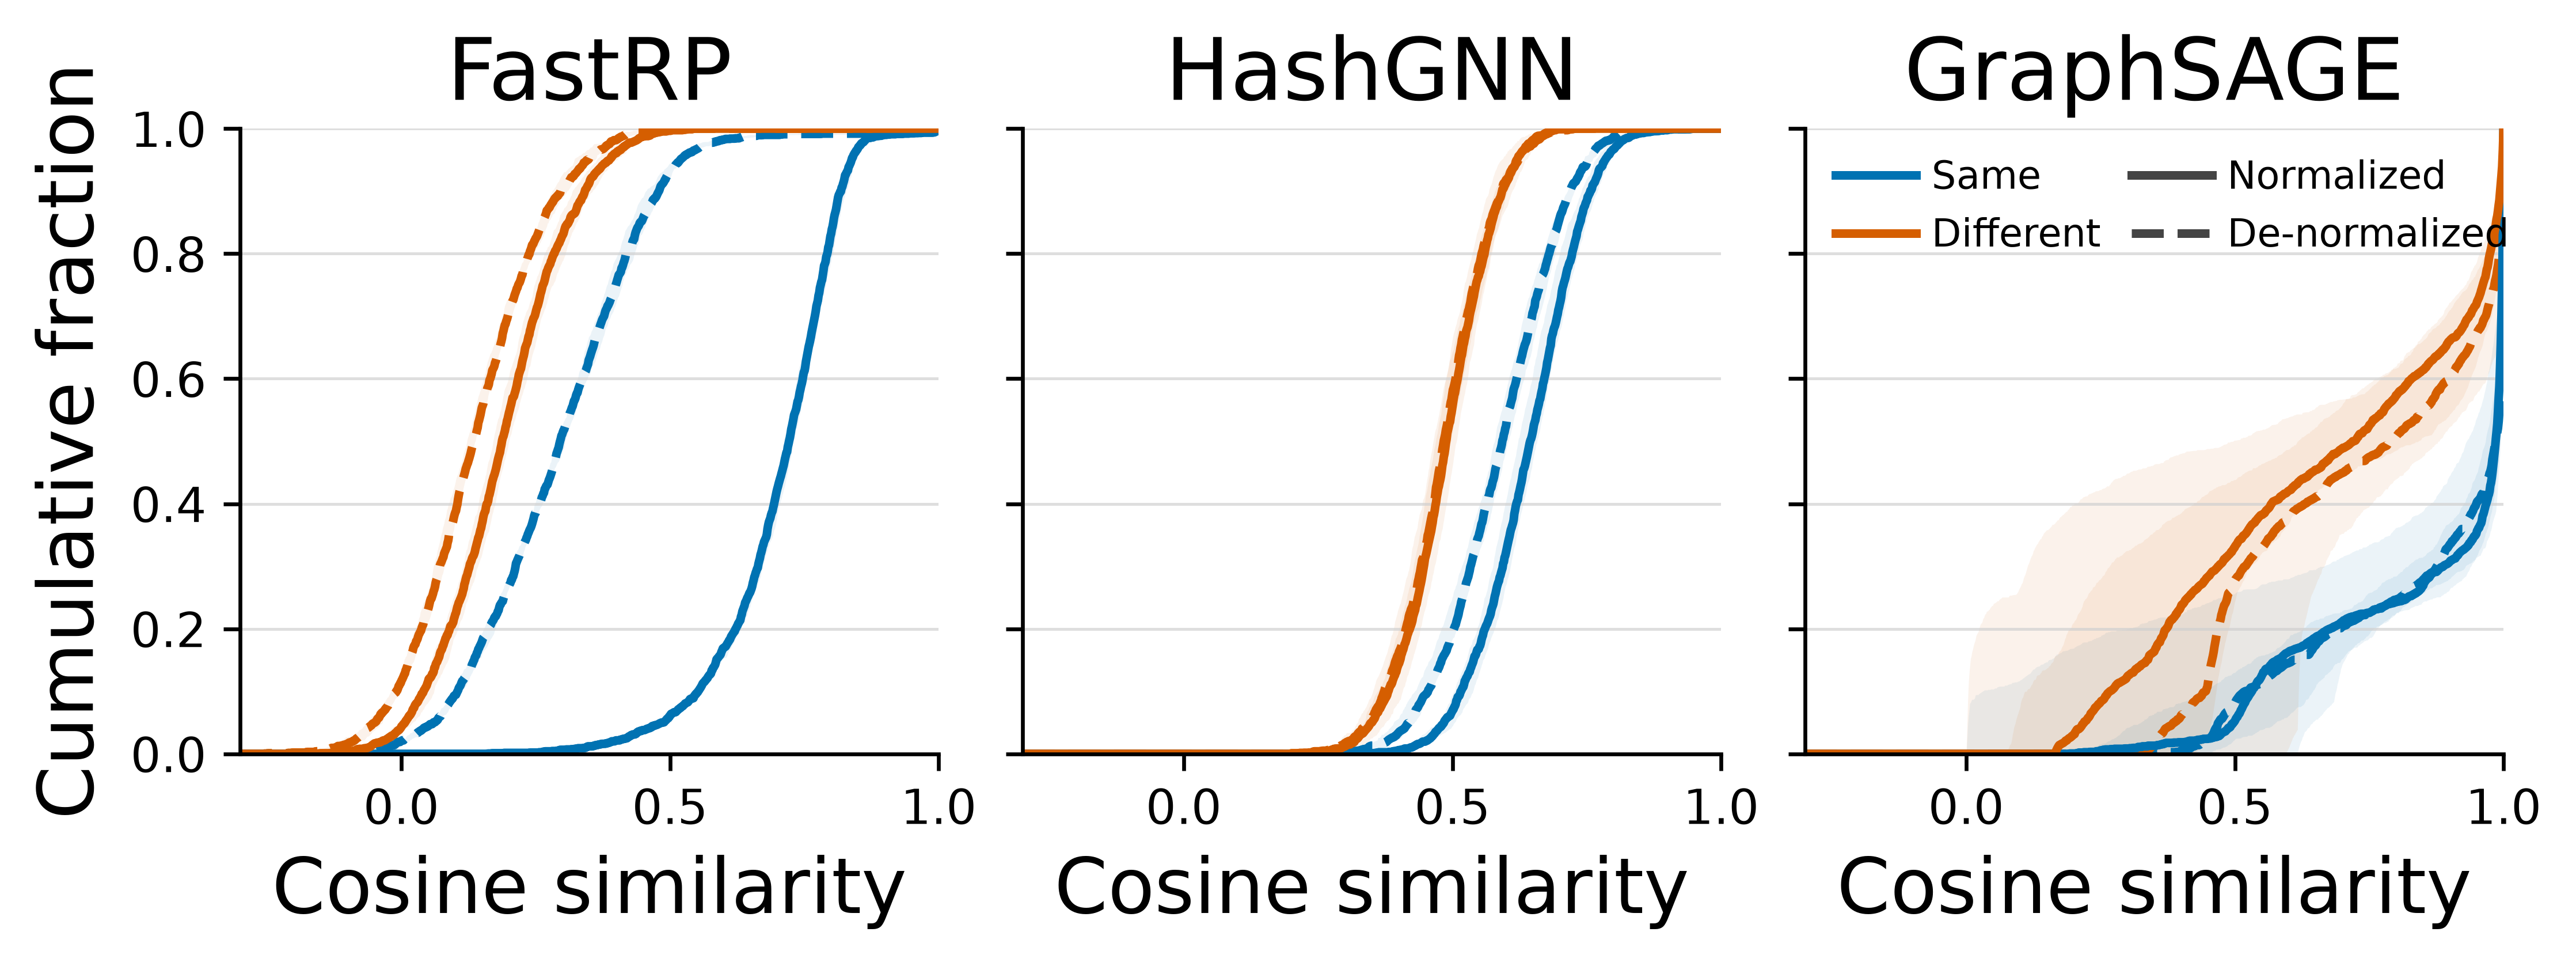
\includegraphics[width=\columnwidth]{figures/experiments/cosine_similarity_ecdf.png}
    \caption{Cosine similarity distributions for
    $\mathit{countries}\rightarrow\mathit{country\_codes}$ on
    \textsf{ADDRESS}.}
    \label{fig:offshore_address_similarity_ecdf}
\end{figure}

Figure~\ref{fig:offshore_address_similarity_ecdf} shows the largest FastRP
change. The horizontal axis gives pairwise cosine similarity, and the vertical
axis gives the fraction of pairs at or below that value; a rightward shift
therefore indicates greater similarity. Two New Zealand address
records have dissimilar original neighbourhoods: one has a single
\texttt{registered\_address} relationship, whereas the other is isolated.
Their similarity is 0.000 in the de-normalized graph. After their country
attributes are moved and both records are linked to the same country node, it
rises to 0.859; records with different countries instead link to distinct
dimension nodes. The shared node thus makes determinant agreement an explicit
structural signal.

%%
%% The next two lines define the bibliography style to be used, and
%% the bibliography file.
\bibliographystyle{ACM-Reference-Format}
\bibliography{sample-base}



\end{document}
